\section{Descrizione del dominio}

Il dominio in cui si sta operando è quello dei fagioli, in particolare quello
delle loro varietà: ogni varietà di fagiolo ha, infatti, specifiche
caratteristiche che la contraddistinguono e che possono essere usate per
identificarle.

Lo studio di questo dominio ha importanti applicazioni pratiche, in 
quanto i fagioli secchi sono uno dei legumi più coltivati al mondo e la loro
coltivazione è fortemente legata alle loro varietà. 
Il processo di classificazione è, però, molto spesso svolto a mano 
da personale addetto e richiede quindi un alto costo e molto tempo.
Un modello di Machine Learning permetterebbe
quindi sia di velocizzare la selezione dei fagioli che di ridurre i costi.

Il dominio analizzato si concentra su sole sette varietà di fagioli, in quanto
quelle più conosciute e interessanti agli autori originali del dataset:
Seker, Barbunya, Bombay, Cali, Dermosan, Horoz e Sira.

\begin{Figure}
    \centering
    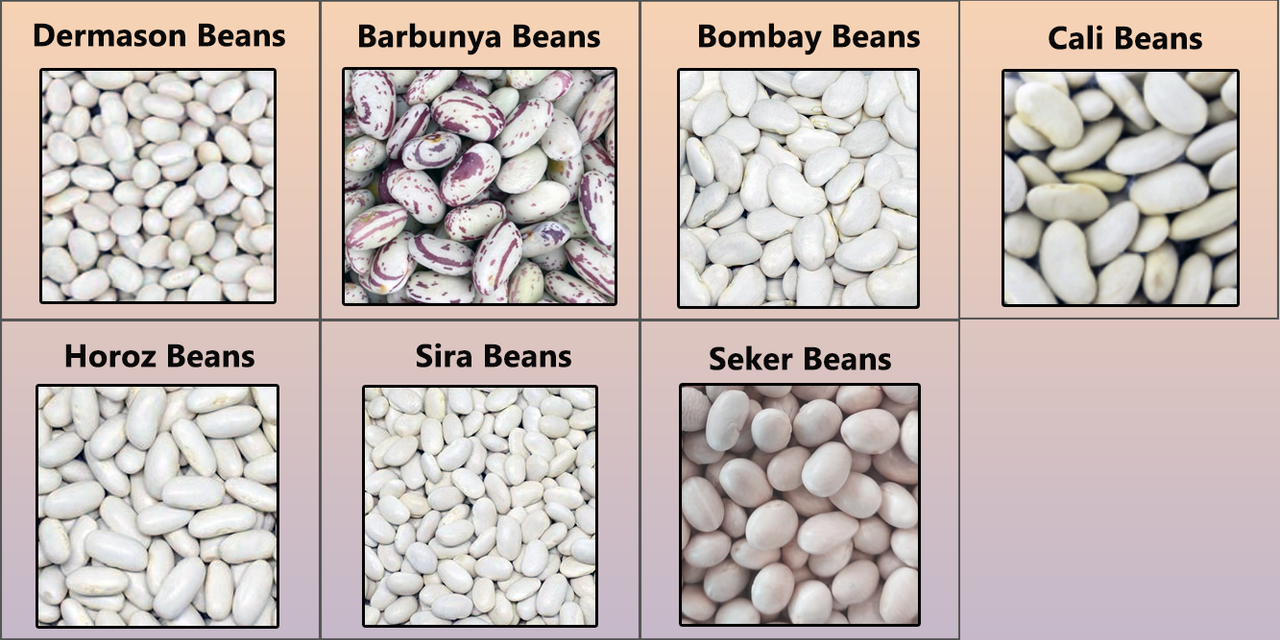
\includegraphics[width=\linewidth]{img/dry_beans.png}
    \captionof{figure}{Varietà di fagioli considerate.}
\end{Figure}